\documentclass[usenames,dvipsnames,tikz]{standalone}
\usepackage{amsmath,amssymb}
\usepackage{xcolor}
\colorlet{tBlue}{RoyalBlue!35!Cerulean}
\colorlet{tRed}{Red}
\usepackage{tikz}
\usepackage{standalone}
\begin{document}
	
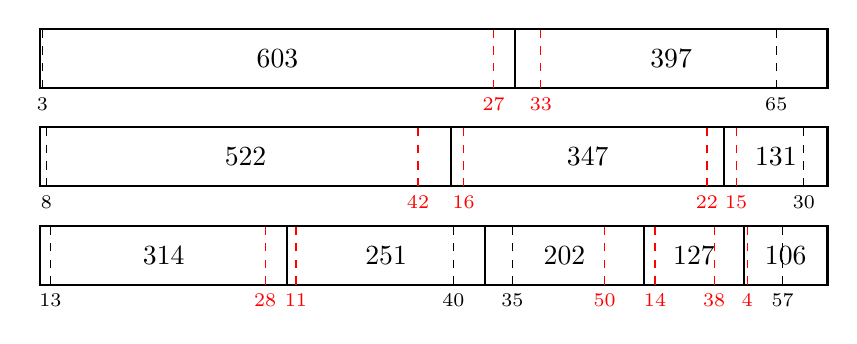
\begin{tikzpicture}
%\draw [help lines] (-1,-2) grid (11,5);
% 1=0.1, 2=0.15, 3=0.2, 4=0.25, 5=0.3
% 6 (3-27), 5 (8-42), 4 (33-65), 4 (16-22), 3 (13-28), 3 (11-40), 2 (35-50), 1 (15-30), 1 (14-38), 1 (4-57).

% BPP
\draw [thick] (0,0) rectangle (10,0.75);
\draw [thick] (0,1.25) rectangle (10,2);
\draw [thick] (0,2.5) rectangle (10,3.25);
%\draw [thick, white] (0,3.75) rectangle (10,4.5);
 
% Bottom row, 314, 251, 202, 127, 106 (13-28 X 11-40, 35-50 X 14-38 X 4-47)
\draw [thick] (3.14,0) -- (3.14,0.75);
\draw [thick] (5.65,0) -- (5.65,0.75);
\draw [thick] (7.67,0) -- (7.67,0.75);
\draw [thick] (8.94,0) -- (8.94,0.75);

\draw [dashed] (0.13,0) -- (0.13,0.75); 
\draw [dashed, tRed] (2.86,0) -- (2.86,0.75);
\node [below] at (0.13,0) {\scriptsize{13}};
\node [below] at (2.86,0) {\textcolor{tRed}{\scriptsize{28}}};

\draw [dashed, tRed] (3.25,0) -- (3.25,0.75);
\draw [dashed] (5.25,0) -- (5.25,0.75);
\node [below] at (3.25,0) {\textcolor{tRed}{\scriptsize{11}}};
\node [below] at (5.25,0) {\scriptsize{40}};

\draw [dashed] (6,0) -- (6,0.75);
\draw [dashed, tRed] (7.17,0) -- (7.17,0.75);
\node [below] at (6,0) {\scriptsize{35}};
\node [below] at (7.17,0) {\textcolor{tRed}{\scriptsize{50}}};

\draw [dashed, tRed] (7.81,0) -- (7.81,0.75);
\draw [dashed, tRed] (8.56,0) -- (8.56,0.75);
\node [below] at (7.81,0) {\textcolor{tRed}{\scriptsize{14}}};
\node [below] at (8.56,0) {\textcolor{tRed}{\scriptsize{38}}};

\draw [dashed, tRed] (8.98,0) -- (8.98,0.75);
\draw [dashed] (9.43,0) -- (9.43,0.75);
\node [below] at (8.98,0) {\textcolor{tRed}{\scriptsize{4}}};
\node [below] at (9.43,0) {\scriptsize{57}};

\node at (1.57, 0.375) {314};
\node at (4.395, 0.375) {251};
\node at (6.66, 0.375) {202};
\node at (8.305, 0.375) {127};
\node at (9.47, 0.375) {106};

% Middle row, 522, 347, 131 (8-42 X 16-22 X 15-30)
\draw [thick] (5.22,1.25) -- (5.22,2);
\draw [thick] (8.69,1.25) -- (8.69,2);

\draw [dashed] (0.08,1.25) -- (0.08,2);
\draw [dashed, tRed] (4.8,1.25) -- (4.8,2);
\node [below] at (0.08,1.25) {\scriptsize{8}};
\node [below] at (4.8,1.25) {\textcolor{tRed}{\scriptsize{42}}};

\draw [dashed, tRed] (5.38,1.25) -- (5.38,2);
\draw [dashed, tRed] (8.47,1.25) -- (8.47,2);
\node [below] at (5.38,1.25) {\textcolor{tRed}{\scriptsize{16}}};
\node [below] at (8.47,1.25) {\textcolor{tRed}{\scriptsize{22}}};

\draw [dashed, tRed] (8.84,1.25) -- (8.84,2);
\draw [dashed] (9.7,1.25) -- (9.7,2);
\node [below] at (8.84,1.25) {\textcolor{tRed}{\scriptsize{15}}};
\node [below] at (9.7,1.25) {\scriptsize{30}};

\node at (2.61, 1.625) {522};
\node at (6.955, 1.625) {347};
\node at (9.345, 1.625) {131};

% Top row, 603, 397 (3-27 X 33-65)
\draw [thick] (6.03,2.5) -- (6.03,3.25);

\draw [dashed] (0.03,2.5) -- (0.03,3.25);
\draw [dashed, tRed] (5.76,2.5) -- (5.76,3.25);
\node [below] at (0.03,2.5) {\scriptsize{3}};
\node [below] at (5.76,2.5) {\textcolor{tRed}{\scriptsize{27}}};

\draw [dashed, tRed] (6.36,2.5) -- (6.36,3.25);
\draw [dashed] (9.35,2.5) -- (9.35,3.25);
\node [below] at (6.36,2.5) {\textcolor{tRed}{\scriptsize{33}}};
\node [below] at (9.35,2.5) {\scriptsize{65}};

\node at (3.015, 2.875) {603};
\node at (8.015, 2.875) {397};


\end{tikzpicture}

\end{document}